\section{Differentially Private Traffic Shaping}
\label{sec:dp}

\todo{The goal of differentially private shaping is to dynamically adjust packet
sizes and timing based on the available data stream, while ensuring that the DP
guarantees hold for any information that an adversary
(\S\ref{subsec:threat-model}) can observe.
}
% \ml{[I suggest moving all that to the end of the DP section for an in-depth
% discussion of the guarantees]
% \am{Clarify that our shaping will provide DP on transmission sizes only. For
% timing we rely on fixed intervals.}
% %
% The adversary can observe sizes, inter-packet intervals, and directions of
% packets in sequences of arbitrary lengths.
% Given these observations, the specific DP guarantee that {\sys} provides is that
% the adversary cannot identify (i) the traffic content (\eg video streams, web
% pages), and (ii) the presence of any one flow between two application
% endpoints.
% %
% We start with a brief primer on DP and its key properties (\S\ref{subsec:DP-background}).
% We then formalize the information available to an adversary observing an
% application's traffic and describe our building blocks for a differentially
% private shaping mechanism in \S\ref{subsec:infromation-bottleneck}.
% We describe our mechanism for sending data based on DP {measurements} in
% \S\ref{subsec:dp-queue-measurements} and prove our guarantees in
% \S\ref{subsec:dp-proof}.
% }
% \subsection{The Shaping Mechanism}
% \label{subsec:infromation-bottleneck}
\Cref{fig:dp-overview} illustrates {\sys}'s DP shaping strategy.
%We denote an application's input packet sequence by
An application's input stream is a packet sequence
$\istream = \{{P^S_1}, {P^S_2}, {P^S_3}, \dots \}$,
%{\as{why do we need a superscript here? it is already defined as $S$.}}
where ${P_i}^S = (l^S_i, t^S_i)$ indicates that the $i$\textsuperscript{th} input
packet in $S$ has length $l^S_i$ bytes and is transmitted at timestamp $t^S_i$.
\ml{We call the total duration of the stream is $\streamduration^S \triangleq
\max t^S_i$.}
Without shaping, an adversary can precisely observe $\istream$ and infer
the content,
% which is any content that is correlated with this stream.
which is correlated with the~stream (\S\ref{subsec:attack-bg}). %\cite{schuster2017beautyburst}.

At a high level, \sys's DP shaping performs DP measurements of the amount
of traffic to send, to adapt the shaped traffic size which preventing data
leakage.
This DP shaping involves three steps (\Cref{fig:dp-overview}).
%First, the preprocessing step transforms an input stream $S$ over a window
%$\window$ into a byte stream, which is
%accumulated in a {\em buffering queue} $\unshapedQ$. (We denote the length of
%$\unshapedQ$ by $\qlen$.) Specifically, as application packets arrive, {\sys}
%extracts the payload bytes and enqueues them into $\unshapedQ$.
\circled{1} As application stream packets $\istream$ arrive, the preprocessing
step extracts the payload bytes and enqueues them into a buffering queue $\buffQ$.
\circled{2} At periodic intervals $T$, the DP shaping algorithm
performs a DP measurement $\qlendpt{T}$ of the size of $\buffQ$, to decide on the
amount of traffic to send.
{\sys} then encrypts and enqueues $\qlendpt{T}$ bytes into the {\em shaped
buffer}, using application bytes from $\buffQ$ when available, and completing
with dummy bytes if required.
\circled{3} Finally, data in the shaped buffer is split into one or more packets
and transmitted to the network. Since these packets are a post-processing of the
DP-shaped buffer, they preserve DP as long as no new dependency on private data
is introduced.
% This last constraint requires the packets' size and transmit time to be selected
% independently of the data.  We describe how {\sys} enforces this constraint in
% \S\ref{sec:implementation}.

We next describe how this design enables \sys's formal DP gurantees.
We start with a primer on DP which, in addition to formal definitions and useful
properties, introduces the three key steps required to provide DP guarantees
(\S\ref{subsec:DP-background}).
We then formalize describe \sys's building blocks for a differentially private
shaping mechanism (\S\ref{subsec:infromation-bottleneck}).
Finally, we prove \sys's shaping algorithm DP guarantees, and discuss the protection
semantics these guarantees offer (\S\ref{subsec:dp-proof}).


% We start with a brief primer on DP and its key properties (\S\ref{subsec:DP-background}).
% We then formalize the information available to an adversary observing an
% application's traffic and describe our building blocks for a differentially
% private shaping mechanism in \S\ref{subsec:infromation-bottleneck}.
% We describe our mechanism for sending data based on DP {measurements} in
% \S\ref{subsec:dp-queue-measurements} and prove our guarantees in
% \S\ref{subsec:dp-proof}.

% To provide DP guarantees, \sys's shaping relies on two key ideas.
% First, it models and controls sensitivity for (potentially long) traffic streams
% in over shorter windows of length $\winlen$ \S\ref{subsec:sensitivity}.
% Second, it uses its {\em buffering queue} primitive to adapt the transmission
% rate to private data $\istream$ while controlling the amount of information
% accessible to an adversary \S\ref{subsec:dp-queue-measurements}.
% This design enables a rigorous DP analysis of {\sys} \S\ref{subsec:dp-proof}.

% \subsection{The Building Blocks}
% \label{subsec:infromation-bottleneck}

% \Cref{fig:dp-overview} illustrates {\sys}'s $(\epsilon,\delta)$-DP
% shaping strategy.
% %We denote an application's input packet sequence by
% An application's input stream is a packet sequence
% $\istream = \{{P^S_1}, {P^S_2}, {P^S_3}, \dots \}$,
% %{\as{why do we need a superscript here? it is already defined as $S$.}}
% where ${P_i}^S = (l^S_i, t^S_i)$ indicates that the $i$\textsuperscript{th} input
% packet in $S$ has length $l_i$ bytes and is transmitted at timestamp $t_i$.
% Without shaping, an adversary can precisely observe $\istream$ and infer
% the content,
% % which is any content that is correlated with this stream.
% which is correlated with the~stream~\cite{schuster2017beautyburst}.

\noindent
\am{Outline:\%\%\%\%\%\%\%\%}
\begin{itemize}
    \item \S 3.1: DP background
    \begin{itemize}
        \item ($\varepsilon, \delta$)-DP definition
        \item Components for building a DP mechanism: neighboring definition,
        query on the dataset and the sensitivity for that query given the
        neighboring definition, noise mechanism
        \item DP properties relevant for {\sys}: post processing, composition,
        robustness to auxiliary knowledge
    \end{itemize}
    \item \S 3.2: Building blocks for a DP mechanism on traffic streams
    \begin{itemize}
        \item Neighboring definition: define window $W$, assumption 1,
        definition 1
        \item Query on streams: call this DP measurement here, define buffering
        queue abstraction, DP interval $T$, explain why $T < W$.
        \item Define the noising mechanism: the additive gaussian noise
        mechanism from shaping overview
    \end{itemize}
    \item \S 3.3: Workflow of {\sys}'s DP shaping and privacy guarantees
    \begin{itemize}
        \item DP workflow: shaping overview (move notations to 3.2)
        \item DP guarantees: ($\varepsilon_W, \delta_W$)-DP through a
        composition of a series of ($\varepsilon_T, \delta_T$)-DP measurements.
        \item How we use DP properties: post processing, composition, and
        robustness to aux. knowledge?
    \end{itemize}
    \item \S 3.4: Proof sketch: Mostly fine, may only require notational
    clarification.
\end{itemize}
\am{End of Outline:\%\%\%\%\%\%\%\%}

\if 0
\subsection{A Primer on Differential Privacy}
\label{subsec:DP-background}
%\as{Comments 4 and 5: Reviewers either specifically asked to have a background
%section or changes that imply the need for a background section. Primier on DP
%need to be before our threat model so we can use DP properties to elaborate on
%our model for attacker (\eg the attacker with auxiliary information).}
%We use Differential Privacy (DP) to quantify the privacy of our shaping
%mechanism.
%DP is a technique originally developed in the context of databases. DP adds
%noise to computations performed on a database (\eg counts, averages) such
%that an adversary cannot learn information about individual database records
%from the DP computation's result.
%Intuitively, a computation is differentially private if changing one record in
%the database does not drastically change the probability of a given result.
% The original definition of DP is specific to statistical databases.
Developed originally for databases, DP is a technique to provide aggregate
results on a database without revealing information about individual database
records.
%
Formally, a randomized algorithm $\mathcal{M}$
%\am{what does ``randomized'' mean?}
is $(\varepsilon, \delta)$-DP
%with respect to a distance metric $\rho$ over databases
if, for all $\mathcal{S} \subseteq \textrm{Range}(\mathcal{M})$ and for all
databases $d, d'$ that differ in only one element, we~have:
%$\rho(d, d') \leq 1$, we have:
\begin{align}
    \label{eq:dp}
    P[\mathcal{M}(d)\in \mathcal{S}] \leq e^{\varepsilon}~P[\mathcal{M}(d')
    \in \mathcal{S}] + \delta
\end{align}
%\mis{I'm not understanding how we're using the dot operator here.}
%\am{It's not a dot operator, but just a scalar product.}
%In other words, a change in a single database record changes the probability of
%any output(s) of $\mathcal{M}$ by at most $e^\varepsilon$.
The parameter $\varepsilon$ represents the {\em privacy loss} of algorithm
$\mathcal{M}$, \ie given a
%\todo{Specifically, a value of $x$ for $\varepsilon$ implies that, given a
% result of $\mathcal{M}$, the probability of identifying whether the input
% database is $d$ or $d'$ is $e^{\varepsilon}$.
result of $\mathcal{M}$, the information gain for any adversary on learning
whether the input database is $d$ or $d'$ is at most $e^{\varepsilon}$
\cite{kasiviswanathan2014semantics}.
The $\delta$ is the probability with which $\mathcal{M}$ fails to bound the
privacy loss to $e^{\varepsilon}$.

The difference between $d$ and $d'$ is called the {\em distance} between the
databases.
It quantifies the granularity at which the DP guarantee applies: given the
result of $\mathcal{M}(d)$, an adversary cannot distinguish whether it was ran
on $d$ or any neighboring database $d'$.
%Enforcing this constraint provably prevents membership inference (learning that
%a specific user contributed data to the database) and reconstruction attacks
%(reconstructing a row of the database) \cite{wasserman2010statistical,
%kasiviswanathan2014semantics, dong2022gaussian}.
%The \todo{strength of the privacy protection} is parameterized by two
%parameters.
%The $\delta$ is the failure probability of mechanism to attain the privacy loss
%(set to an appropriately small number).}
%\am{provide accurate intuition of $\varepsilon$ and $\delta$.}
%For both parameters, smaller means more private.
Traditionally, this distance is defined as the number of records that differ between $d$ and $d'$, and the DP guarantee is over any neighboring databases (at distance one).
However, DP extends to other neighboring definitions based on distance metrics for use in specific settings \cite{chatzikokolakis2013broadening, lecuyer2019certified}, which we leverage in \sys.
% The first step for making an algorithm DP is to formalize this neighboring definition (\S\ref{subsec:infromation-bottleneck}).
In {\sys} we also use a different distance, and hence neighboring, definition to define DP guarantees over dynamic traffic streams (\S\ref{subsec:building-blocks}).

\ml{[Introducing the notion of sensitivity, which we need before we can detail]
The most common DP mechanisms, which we use in {\sys}, make a computation DP by
adding noise to the non-private result. This noise needs to be scaled to the
{\em sensitivity} of the computation, which is the worst possible change to the
resut when running the mechanism on two neighboring databases $d$ and $d'$
(details in \S\ref{subsec:building-blocks}).
% The second and third steps of making an algorithm DP are to bound the
% sensitivty of the computation, and add noise scaled to this sensitivity
% (\S\ref{subsec:dp-queue-measurements}).
}

Our shaping mechanism relies on three fundamental properties of DP.
First, DP is resilient to post-processing: given the result $r$ of any
$(\varepsilon, \delta)$-DP mechanism $\mathcal{M}$, any function $f(r)$
%$(\varepsilon, \delta)$-DP mechanism $r \sim \mathcal{M}$, any function $f(r)$
of the result is also $(\varepsilon, \delta)$-DP.
%\am{Do we need to say that the function must be independent of input data?}
%\as{The only input that function receives is the result. I don't think we need
%to mention the independence of function again.}
As a result, any computation or decision made on a DP result is still DP with
the same guarantees.
Second, DP is closed under adaptive sequential {\em composition}: the combined
result of two DP mechanisms $\mathcal{M}_1$ and $\mathcal{M}_2$ is also DP,
though with higher losses ($\varepsilon$ and $\delta$).
We use the R\'enyi-DP definition~\cite{mironov2017renyi} to achieve simple but
strong composition results and subsequently convert the results
back to the standard DP definition.
%\am{$\leftarrow$ unclear statement.}
%
Third, DP is robust to auxiliary information: the guarantee from \Cref{eq:dp}
holds regardless~of any side information known to an attacker.
\update{Therefore, attacker's knowledge of shaping mechanism does not affect its privacy guarantees}
% \am{Can we provide some more explanation of this?}
That is, an attacker knowing or controlling part of the database cannot extract
more knowledge from a DP result than without this side information.
%\as{I found it also hard to explain. The most intuitive explanation of auxiliary
%information I've ever seen is from Aaron Roth's book: DP guarantees ensures that
%anything is known about the input of the mechanism after seeing the output of
%mechanism was known before seeing the output of the mechanism, meaning that the
%output does not add to the prior knowledge of adversary, regardless of its level
%of information, beyond the privacy bounds defined by DP. For example, if before
%seeing the output, the adversary knows that a user is going to watch a video of
%a cat or a video of a dog, after seeing the output, the probability that user
%watched either of them is still bounded by DP.}

% In this section, we describe our conceptual shaping strategy. In the next
% sections, we describe the design of our complete system that uses the strategy
% while shaping actual traffic.

%Shaping involves transmitting packets such that their sizes and timing do not
%reveal secrets.
%The goal of our DP traffic shaping mechanism is to dynamically adapt the data
%transmission rate based on the available data stream, while ensuring that the DP
%guarantees hold for any information that an adversary can observe.
%The design of our traffic shaping algorithm relies on three key steps.
%%
%First, we formalize the information available to an attacker observing an
%application stream, which is all information such as packet sizes or timing at
%the finest granularity of observation.
%We propose to use a buffering queue to collapse all this information into a
%sufficient statistic to adapt {\sys}'s transmission rate: the size of data in
%the queue waiting to be transmitted through our shaping mechanism
%(\S\ref{subsec:infromation-bottleneck}).
%%
%Second, we show how to perform {\em DP measurements} of our buffering queue, in
%order to adapt \sys's transmission rate with DP guarantees.
%Indeed, we show that under natural constraints on the transmission rate
%decision mechanism, the change of queue size is bounded, allowing us to perform
%DP measurements (\S\ref{subsec:dp-queue-measurements}).
%%
%Third, we describe our decision mechanism for sending data based on DP
%decisions, which completes our DP shaping mechanism
%(\Cref{alg:dp_shaping_mechanism}).
%Intuitively, we can use DP queue measurements and public information such as
%network conditions to decide the amount of data to transmit.
%Transmissions contain queued data when some is available, and dummy data
%otherwise.
%The stream observed by any attacker is a post-processing of the DP queries
%issued on the queue (depends on the private data only through the DP
%measurements), and is hence DP.
\fi

\begin{figure}[t]
    \centering
    %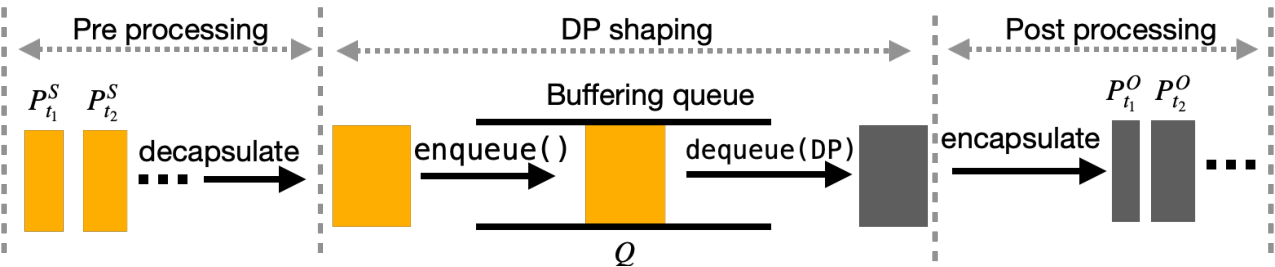
\includegraphics[width=\columnwidth]{figures/DPshaping_concept_vertical.pdf}
    %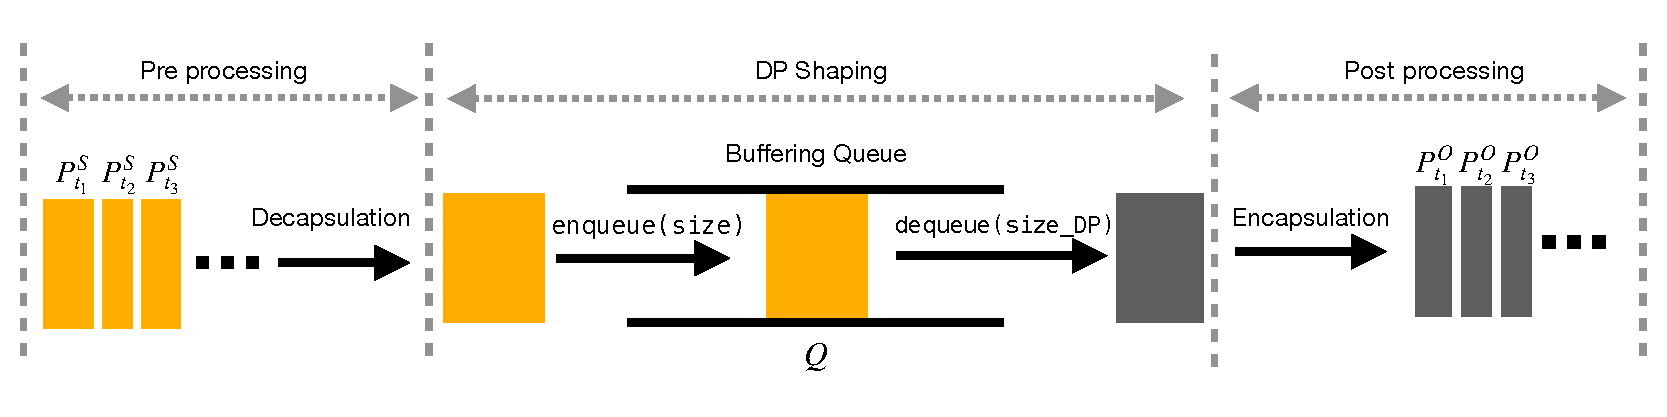
\includegraphics[width=\columnwidth]{figures/DPshaping_concept_horizontal.pdf}
    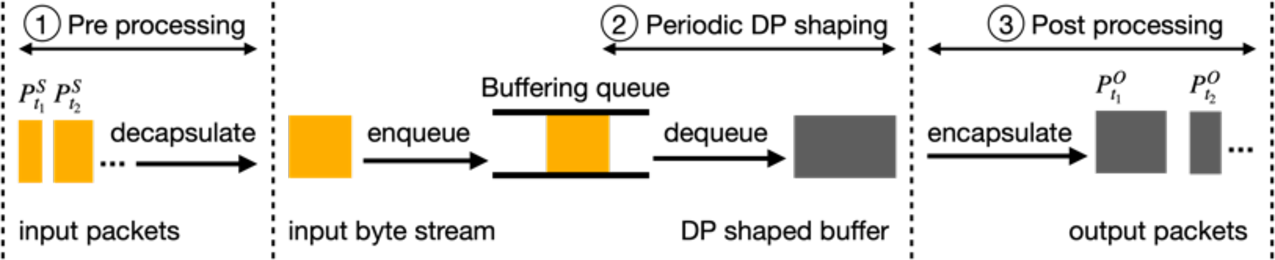
\includegraphics[width=\columnwidth]{figures/dp-overview.pdf}
    \caption{Overview of DP shaping}
    \label{fig:dp-overview}
\end{figure}

%\paragraph{Goal.}
%The design of our traffic shaping algorithm relies on three key steps.
%The rest of this section is organized as follows.
%In \S\ref{subsec:infromation-bottleneck}, we formalize the information available
%to an attacker observing an application stream, which is the sequence of sizes,
%inter-packet intervals, and directions of packets at the finest granularity of
%observation.
%%We propose a primitive of a {\em buffering queue} to collapse all this
%%information into a sufficient statistic to adapt {\sys}'s transmission rate:
%%the
%%size of data in the queue waiting to be transmitted through our shaping
%%mechanism.
%%
%In \S\ref{subsec:dp-queue-measurements}, we describe our decision mechanism for
%sending data based on DP decisions.
%%We show how to perform {\em DP measurements} of our buffering queue, in
%%order to adapt \sys's transmission rate with DP guarantees.
%%We show that under natural constraints on the transmission rate decision
%%mechanism, the change of queue size is bounded, allowing us to perform DP
%%measurements.
%%(\Cref{alg:dp_shaping_mechanism}).
%%Intuitively, we can use DP queue measurements and public information such as
%%network conditions to decide the amount of data to transmit.
%%Transmissions contain queued data when some is available, and dummy data
%%otherwise.
%%The stream observed by any attacker is a post-processing of the DP queries
%%issued on the queue (depends on the private data only through the DP
%%measurements), and is hence DP.
%%
%Finally, in \S\ref{subsec:dp-proof}, we provide a proof sketch for the DP
%guarantees of our shaping mechanism.

%{\as{I don't think we should summarize the intro of DP section into only one
%paragraph. We should give a summary of section here, explaining why we think DP
%shaping is a good idea and how it works Intuitively. More importantly, I think
%we need to  }}
%Specifically, given an application with a corpus of objects, the DP shaping
%ensures that each pair~of {\em neighbouring} objects---whose sizes are within a
%bounded distance---is indistinguishable under DP notion from the observations of
%their traffic shape.
%We denote the maximum distance between any pair of application objects by
%$\ssens$.
%
%Intuitively, {$\sys$} aims to ensure that a stream $S$ is indistinguishable (in
%the DP sense) from a neighboring stream $S'$ by observing the shaped traffic.

\subsection{The Building Blocks}
\label{subsec:building-blocks}
% \subsection{The Sensitivity for DP Measurements}
% \label{subsec:sensitivity}

The main primitive in \sys's DP adaptive shaping is a DP measurement of the
buffering queue ($\buffQ$) size.
As discussed in \S\ref{subsec:DP-background}, making a measurement DP requires
three steps: defining a granularity of protection through a neighboring
definition, bounding the sensitivity of the computation, and adding noise to the
computation result.
We describe the key ideas in \sys's design that make this possible.

\paragraph{Neighboring Definition.}
Recall that the neighboring definition formalized the level of granularity at which
the DP guarantee applies. Intuitively, neighboring streams are undistinguishable based
on the results of DP measurements.
%
% An application stream $\istream$ includes information at the packet level.
To formalize a meaningful neighboring definition for  (potentially long) traffic
streams that include information at the packet level, we first focus on windows
of fixed length $\winlen$.
An input sequence over window $j$ is a finite~sub\-sequence $S_{j} \subset S$,
such that $S_{j} = \{ P^S_i~|~P^S_i \in S~and~t_i \in j \}$.
% {\sys}'s DP guarantees \todo{cover} all (overlapping) windows up to size
% $\winlen$.
We then define a meaningful distance between any pair of streams, and the
associated neighboring definition, over any windows of length $\winlen$:

\begin{definition}
Two streams $S$ and $S'$ are neighbors if, for any window $j$ of length
  \todo{$\winlen$ or less}, the L1-norm distance between sub\-sequences  $S_{j}$
  and $S_{j}'$ is at most~$\ssens$ bytes, \ie ${\norm{~S_{j} - S_{j}'~}}_1 \leq \ssens$.
\label{def:neighboring-streams}
\end{definition}

$\ssens$ is the max L1-norm of the difference between a pair of application
streams in traffic bytes, over any window of length up to $\winlen$.
That is, two streams are neighbors if, over any window of length $\winlen$ or less,
the absolute difference in the amount of traffic they send is less than $\ssens$.
\as{I don't think we want to say \textbf{absolute difference} because the absolute difference only captures difference in size of two flows. The norm difference is the sum of absolute difference between every two corresponding pairs of burst sizes, and it captures temporal difference.}
We utilize the L1-norm (the sum of absolute values) as our distance metric
to quantify the dissimilarity between two traffic streams, as it captures
differences in both traffic size and \todo{temporal alignment.}

The window length $\winlen$ and neighboring size $\ssens$ are both configuration
parameters, which are set before the start of an application's transmission.
In practice, $\winlen$ would be in the order of a few seconds.
%
% \ml{Add discussion about an upper bound for $\ssens$ here, and say we can also
% use something smaller.}
%
% We will see that despite this restriction in the neighboring definition, we can
% quantify \sys's DP guarantees for streams of any length.
\todo{$\ssens$ quantifies the strength of the neighboring definition, and hence of the
DP guarantee. Setting $\ssens$ to the line rate throughput times window length
$\winlen$ means that all streams that can possibly be sent are neighbors with each
other.
This yields a strong DP definition making any stream indistinguishable, but high
overheads (\S\ref{}).
Using domain knowledge to set a lower $\ssens$---such as based on the typical
difference of traffic between video streams of interest over windows of length
$\winlen$, or the maximum size of traffic for a web request---reduces overhead
while still providing meaningful guarantees.}


\paragraph{Bounding Sensitivity.} The second step in providing DP measurements
is to bound the sensitivity of the computation we want to make private. Remember
that we aim to measure the state of traffic to adapt the amount of shaped traffic
we send.
Since the sensitivity is the worst case change in result between two neighboring
streams, we need to reason about the worst case change to any measurement we want
to make, when performing this measurement on two adjacent streams.
We defined adjacent streams in terms of the difference of amount of traffic sent
over time, but there could be large differences in packetization, making it
difficult to bound the impact on any measurement.
%
\sys's key idea is to use the primitive of a {\em buffering queue} to control
the maximum information accessible by a measurement, and hence the sensitivity
of the computation.
Conceptually, {\sys} extracts bytes from the input stream, $\istream$, and
enqueues them in the buffering queue $\buffQ$.
We denote the number of bytes present in $\buffQ$ (\ie length of the queue) by
$\qlen$.

With this primitive in place, we are now ready to define our DP measurement and
analyse its sensitivity. We use subscript $T$ to denote measurement specific
quantities.
As $\qlen$ is the amount of application data waiting in $\buffQ$ to be sent, we
would ideally want {\sys} to move $\qlen$ bytes from $\buffQ$ to the shaped
buffer, for it to be sent over the network.  Hence {\sys} measures $\qlen$, with
DP to provide privacy guarantees. To make the measurement DP we need to bound
$\qsens$, the sensitivity of $\qlen$, which is the maximum difference in the
queue length $\qlen$ that can be caused  by changing one application stream to
neighboring one.
Formally, consider two alternative neighboring streams $\istream$ and
$\istream'$ passing through the queue.
Suppose that when transmitting $\istream$ (similarly $\istream'$), the
queue length at time $t$ is denoted by $\qlent{t}$ (respectively $\qlent{t}'$).
Then, assuming without loss of generality that $\streamduration \geq
\streamduration'$:
\setlength{\abovedisplayskip}{0pt}
\begin{equation}
    \qsens = \max_{t = 0}^{\streamduration}~\max_{\istream,
        \istream'} | \qlent{t} - \qlent{t}' |
    \label{eqn:ssens}
\end{equation}

Bounding $\qsens$ is still challenging thought, as our neighboring definition
only bounds the difference in traffic between two streams over any window of
length $\winlen$.
For long streams with $\streamduration >> \winlen$, differences between
$\istream$ and $\istream'$ can accumulate and grow unbounded.
To bound sensitivity, {\sys} relies on the key assumption that
\todo{the tunnel can always transmit all incoming data from
application streams within any $\winlen$-sized time window.}
\ml{Is it the tunnel, or just the buffering queue?}
In other words, we assume that:
%is that the tunnel can handle all incoming data from application streams within
%$\winlen$-sized window of time.
%Specifically, we make the following assumption:
\begin{assumption}\label{assumption:window}
  All bytes enqueued \todo{prior to or} at time $t$ are transmitted by time
  $t+W$.
\end{assumption}
We explain how to realize this assumption in a tunnel design in
\S\ref{sec:design}.
\ml{Do we explain that somewhere? Should we actually explain it here (dropping
the queues) so that we can discuss the $W$ and $T$ tradeoff in this section?}
%
Intuitively, this assumption caps the accumulation of traffic differences in
$\buffQ$ to the maximum difference over $\winlen$, and we can bound the
sensitivity of $\qsens \leq \ssens$. We defer the proof, which requires
accounting for DP noise, to \S\ref{subsec:dp-proof},
Proposition~\ref{prop:sensitivity}.

\paragraph{Adding Noise.}
With sensitivity bounded at $\ssens$, we are now measure $\qlen$ with DP using
an additive noise mechanism, which entails sampling noise $z$ from a DP
distribution and computing the DP buffer queue length as $\qlendpt{k} \triangleq
\qlent{k} + z$.
Specifically, {\sys} uses the Gaussian mechanism, in which
The noise $z$ is sampled from a centered normal distribution
$z \sim \mathcal{N}\big(\mu,~\sigma^2\big)$, where the variance is parameterized by
$\epsilon_\dpintvl$, $\delta_\dpintvl$, and~$\qsens$:
$\sigma^2 = \frac{2\qsens^2}{\varepsilon_\dpintvl^2}\ln(\frac{1.25}{\delta_\dpintvl})$.
Under this noise distribution, one measurement is \mbox{$(\epsilon_\dpintvl,
\delta_\dpintvl)$-DP}.


\subsection{The Shaping Mechanism}
\label{subsec:dp-queue-measurements}

We can now combine the building blocks into an end-to-end adaptive shaping
mechanism, shown on \Cref{fig:dp-overview} and detailed in \todo{Algorithm
\ref{}}\ml{TODO: it should show a function for depacketization; one for periodic
DP measurements + queue change; one that sends from the shaped buffer.}.
There are three main steps.
First, we can see the de-packetization of applications traffic, which is queued in the
buffering queue (\circled{1}, ll. \todo{x-x}).

Second, adaptivity to application traffic comes from periodic DP measurements
$\qlendp$ of the buffering queue size at intervals $T$.
DP measurements are used to decide how much data to dequeue from the buffering
queue, encrypt, and enqueue into the shaped buffer to be sent over the network
(\circled{2}, ll.  \todo{x-x}).
Enqueueing data into the shaped buffer creates a sequence of states for the
shaped buffer $\{(T, \bar{L}_1), (2T, \bar{L}_2), (3T, \bar{L}_3) \dots \}$.
\ml{can we get better notation for this?}
Although this sequence is not technically observable by an adversary, this is
where we prove our DP guarantees using DP composition over DP measurements
performed while the stream is running (\S\ref{subsec:dp-proof}).
\todo{We will see that the DP property holds as long as the enqueueing times are
selected independently of the data.  We describe how {\sys} enforces this
constraint in a best effort fashion in \S\ref{sec:implementation}.}

Finally, data from the shaped buffer is sent over the network, transmitted as a
packet sequence denoted by $\ostream = \{{P^O_1}, {P^O_2}, {P^O_3} \dots \}$,
which is observable by an adversary (\circled{3}, ll.  \todo{x-x}).
Since these packets are a post-processing of the DP-shaped buffer, the
post-processing property of DP ensures that they preserve DP as long as no new
dependency on private data is introduced.

\begin{algorithm}
  \caption{DP Shaping Mechanism \as{I'm not sure that we want to mention dummy and data here. It sounds more like implementation details but without it the pseudocode would be inaccurate. The other problem is that our system is by definition multithreaded, where the enqueue function and DP measurement cannot happen in the same loop. Do we want to mention that?}}
  \KwData{$P_{t_1}^S, P_{t_2}^S, \dots $}
  \KwResult{$P_{t_1}^O, P_{t_2}^O, \dots $}
  
  \While{True}{
    \texttt{sleep($T$)}\;
    \texttt{enqueue($Q_{DP}, \{P_{t_1}^S, P_{t_2}^S, \dots\}$)}\;
    $\qlendp$ =  \texttt{DP\_measurement($Q_{DP}$)}\;
    $R$ = \texttt{dequeue($Q_{DP}, \min(\qlendp, \qlen)$)}\; 
    $D$ = $\qlendp - R$\;
    \texttt{enqueue($Q_{QUIC}, R + D$)}\;
    $P_{t_1}^O, P_{t_2}^O, \dots $ = \texttt{QUIC\_send($Q_{QUIC}$)}}\;
  
\end{algorithm}
 
% \begin{figure}
%   \centering
%   \begin{minipage}{0.8\linewidth}
%     \begin{algorithm}H]
%       \caption{DP Shaping Mechanism}
%       \KwData{$P_{t_1}^S, P_{t_2}^S, \dots $}
%       \KwResult{$P_{t_1}^O, P_{t_2}^O, \dots $}

%       \While{True}{
%         \texttt{sleep($T$)}\;
%         \texttt{enqueue($Q_{DP}, \{P_{t_1}^S, P_{t_2}^S, \dots\}$)}\;
%         $\qlendp$ =  \texttt{DP\_measurement($Q_{DP}$)}\;
%         $R$ = \texttt{dequeue($Q_{DP}, \min(\qlendp, \qlen)$)}\; 
%         $D$ = $\qlendp - R$\;
%         \texttt{enqueue($Q_{QUIC}, R + D$)}\;
%         $P_{t_1}^O, P_{t_2}^O, \dots $ = \texttt{QUIC\_send($Q_{QUIC}$)}}\;
%     \end{algorithm}
%   \end{minipage}
%   \caption{Description of the DP Shaping Mechanism}
% \end{figure}



\paragraph{Impact of DP Shaping on Performance.}
\ml{[TODO: with at least this info taken from other places while moving things]
%
Specifically, large windows lead to high-latency bursty traffic.
\shepherd{To reduce latency and burstiness}\as{comment 1.b: we should explain how does having two windows recduce the burstiness and why we cannot make W as small as T}, {\sys} further splits windows into
smaller intervals of length $\dpintvl$ and samples noise at the beginning of
each interval.
\todo{In absence of shaping, the queue length corresponds to the amount of
    unshaped traffic transmitted in an interval of $\dpintvl$.}
The privacy loss over a window is now defined by applying DP composition
on the privacy loss of individual intervals.
%
The privacy loss ($\varepsilon_{\winlen}$) and bandwidth overheads of the DP
shaping (represented by $\sigma_\dpintvl$, \ie the standard deviation of the
noise distribution function) depend on
$\winlen$, $\ssens$,
%$\varepsilon_{\dpintvl}$, $\delta_{\dpintvl}$,
and the number of intervals $\varnumupdates = \numupdates$ in $\winlen$.
Additionally, the latency overheads depend on $\dpintvl$.
Note that for a specific value of $\ssens$ and $\varnumupdates$, the DP guarantee
$\varepsilon_{\winlen}$ is fully specified by $\sigma_\dpintvl$, and remains the same even at
different time scales.
That is, scaling $\winlen$ and $\dpintvl$ proportionally does not change the
privacy and overhead costs.
%{\as{We are not sure about this, the latency can be affected by the amount of
%noise in extreme scenarios}}
We analyze the impact of different choices for these parameters on
the privacy guarantees and overheads in \S\ref{sec:eval}. Here, we focus on a
formal model of the DP guarantees.
}


\subsection{Privacy Guarantees}
\label{subsec:dp-proof}
%\as{I think we need to change the title of this section as it is not the proof
%but also proposing our guarantees. I suggest the title: "Privacy guarantees".}
At a high level, analyzing the  ($\varepsilon_{\winlen}, \delta_{\winlen}$)-DP
guarantee of the overall shaping mechanism requires two steps: (i) showing that
the difference in the buffering queue length is bounded for neighboring streams
for all transmissions of the streams (Prop. \ref{prop:sensitivity}), and (ii)
composing the DP cost of each measurement over the intervals defining a window
of length $\winlen$ (Prop. \ref{prop:dp}).
%\todo{(i) two neighboring streams in windows of length $\winlen$ are neighbors
%during all transmit intervals of length $\dpintvl$, and (ii) the total privacy
%loss composed over all transmit intervals within a window amounts to the privacy
%loss defined over the entire window.}
%\am{Verify wording.}
%\as{I think the wording is wrong for both points. We need to show that
%difference in queue lengths are bounded. Then the second point naturally follows
%by composition.}
%(i) the neighboring definition over the buffering queue length over intervals
%$\dpintvl$ implies neighboring definition

%Formally, {$\sys$} offers the following guarantee:
We first show that the sensitivity of each measurement $\qsens$ is at most the
window sensitivity $\ssens$:
\begin{proposition}\label{prop:sensitivity}
    {$\sys$} enforces $\qsens \leq \ssens$.
\end{proposition}

\begin{proofsketch}
  Consider any two streams $S_j$ and $S_j'$, as in \Cref{eqn:ssens}.
  The proof proceeds in two steps. First, under \Cref{assumption:window},
  streams can accumulate queued traffic for at most {$\winlen$}, so two
  different streams can create a difference $|\qlent{k} - \qlent{k}'|$ of at
  most $\ssens$.
  Second, dequeuing can only make two different queues closer: Consider
  measurement time $k$, with queue lengths $\qlent{k} > \qlent{k}'$ (the
  opposite case is symmetric).
  For a DP noise draw $z$, we have $\qlendpt{k} > \qlendpt{k}'$. Since shaping
  sends at least as much data under $\qlendpt{k}$ as under $\qlendpt{k}'$,
  but no more than $\qlendpt{k} - \qlendpt{k}'$, after dequeuing we have
  $|\qlent{k+1}' - \qlent{k+1}| \leq |\qlent{k}' - \qlent{k}|$.
  In summary, the maximum queue difference under two different streams
  $\qsens$ can grow to at most $\ssens$ due to data queuing, and dequeuing only
  decreases that difference, and hence $\qsens \leq \ssens$.  The complete proof
  is in \S\ref{appendix:dp}.
\end{proofsketch}

We can then reason about DP guarantees over intervals of length $\dpintvl$ in
order to achieve the privacy loss for the entire window of length $\winlen$.
%
\ml{[TODO Mathias] make notation consistent: here we want only the stream length
and then use W as a numerical application. This will show that we can compose over time}
Formally, we have:
\begin{proposition}\label{prop:dp}
  {$\sys$} enforces $(\varepsilon_{\winlen}, \delta_{\winlen})$-DP, with
  $\varepsilon_{\winlen}, \delta_{\winlen} \triangleq
  \textrm{DP\_compose}(\varepsilon_T, \delta_T, \numupdates)$.
\end{proposition}

\begin{proof}
By Prop. \ref{prop:sensitivity}, the sensitivity of each measurement is at most
  $\ssens$.
%\am{I thought the sensitivity is already defined in \Cref{eqn:ssens}.}
By the Gaussian DP mechanism, the measured queue size $\qlendpt{k}$ in each
interval $k$ of length $\dpintvl$ is $(\varepsilon_{T}, \delta_{T})$-DP.
% Over a time window of length $\winlen$, {\sys} will sample noise
% $\numupdates$ times.
Using DP composition over $\numupdates$ $(\varepsilon_{T}, \delta_{T})$-DP
measurements, and the fact that $\ostream$ is a post-processing of DP
measurements, yields the ($\varepsilon_{\winlen}, \delta_{\winlen}$)-DP over
any $\winlen$ length window.
% By using R\'enyi algorithm for DP\_compose(), we get $\varepsilon$,
% $\delta$ that correspond to ($\varepsilon_{\winlen}, \delta_{\winlen}$)-DP
% definition over $\winlen$ windows.
%\todo{Thus, the proof concludes with the application of DP composition.}
%\am{I am not sure how the last line follows from the second last line: what does
%it mean say proof concludes with application of DP composition.}
%\as{It is just the way of saying that compositions is applied here and privacy
%parameters, $\varepsilon_W, \delta_W$ are result of it.}
\end{proof}
We use R\'enyi-DP composition on the Gaussian mechanism for
$\textrm{DP\_compose()}$.
%If $\winlen$ is larger than all traffic streams, {$\sys$} enforces
%$(\varepsilon_{\winlen}, \delta_{\winlen})$-DP over all streams going through he
%shaped tunnel. \am{Not sure what the previous statement is trying to
%say.}{\as{I also think maybe it is better to remove it}}
Note that the overhead (\ie noise added) due to
DP does not depend on the number of streams: the overhead is the same regardless
of the number of streams transmitted through the buffering queue simultaneously.


%\smallskip\noindent
\paragraph{Summary.}
By buffering all data in a queue, and periodically deciding the size of the data
to send over the network with a DP measurement, \sys's shaping algorithm
makes the shape of traffic (volume of data sent over time) DP with regards to
the application's original traffic sequence.
%The DP shaping algorithm ensures that an adversary cannot trace the observed
%packet sizes on the network back to the packet sizes in the application's
%original sequence.
% The DP shaping algorithm makes \ml{the amount of traffic \sout{the packet sizes}
% output} on the network independent of (DP with regards to) the amount of traffic
% in the application's original sequence, in each window of size $\winlen$.
% of the packet sizes in the application's
% original sequence.
% \ml{[this is wrong without the later timing things I think, shoule remove? Or at
% least should be refined, I'm not too sure what the goal is here] Furthermore,
% due to the periodic execution of algorithm and the subsequent DP post processing
% property, the timing of output packets is also independent of the packet timings
% in the original sequence.}
Thus, as long as no observable characteristics of the traffic directly depend on
application secrets (the original traffic sequence), the observable outbound traffic
is DP.
% Thus, the algorithm ensures that the shape of the outbound traffic of an
% application is independent of application secrets.

%\am{The proof of the DP guarantees of the algorithm is provided in the
%appendix. Can we prove that constant timing intervals + differentially privacy
%on size = differentially privacy on the overall traffic shape?}

\ml{\paragraph{Interpretation} Let's add something on interpreting the guarantees and what they mean here: hidding any marginal change of size sensitivity (presence + content); composition over time; group composition for larger sensitivity.}
\ml{[This is from the intro]
\am{Clarify that our shaping will provide DP on transmission sizes only. For
timing we rely on fixed intervals.}
%
The adversary can observe sizes, inter-packet intervals, and directions of
packets in sequences of arbitrary lengths.
Given these observations, the specific DP guarantee that {\sys} provides is that
the adversary cannot identify (i) the traffic content (\eg video streams, web
pages), and (ii) the presence of any one flow between two application
endpoints.
}
\ml{
{\sys}'s DP guarantees \todo{cover} all (overlapping) windows up to size
$\winlen$, and composes over larger windows.
}
\ml{Here we want to discuss group composition and the neighboring definition in general}

%%%%%%%%%%%
%% old text
%%%%%%%%%%%
% \paragraph{Unshaped queue.}
% We model an abstract queue, {$\unshapedQ$}, which holds the unshaped input byte
% stream of an application and supports two operations: enqueue and dequeue.

% \paragraph{Neighboring queue states.}
% We define the queue state, ${\unshapedQ}_{\tau}$, as the amount of traffic
% inside ${\unshapedQ}$ at time $\tau$. We call two queue states, ${\unshapedQ}_{\tau}$
% and ${\unshapedQ}'_{\tau}$, neighbor queue states if and only if we have:
% \begin{equation}\label{equ:queue-neighboring}
        % |{\unshapedQ}_{\tau} - {\unshapedQ}'_{\tau}| \leq D_q \;(bytes)
% \end{equation}
% where $D_q$ is a parameter in our system.


% \paragraph{Query function and sensitivity.}
% We define a query function on the queue state ${\unshapedQ}$,
% $f({\unshapedQ}_{\tau})$, as a function that returns the
% size of the queue at time ${\tau}$. The sensitivity of the function $f$ is given~by:
% \begin{equation}
% \Delta_1 f = \max_{Q, Q'} \| f(Q_{\tau}) - f(Q'_{\tau}) \|_1 =  \max_{Q, Q'} \| Q - Q' \|_1 = D_q
% \end{equation}
% Here, $\Delta_1 f$ captures the magnitude by which the size of queue can change
% from one stream to another.  In fact, {\sys}'s shaping strategy guarantees that
% the queue size cannot be accurately ascertained by an attacker.  At this point,
% we have all necessary building blocks to propose our differentially private
% shaping algorithm.

% \paragraph{From queues to traffic streams.}

% The definition presented in \Cref{equ:queue-neighboring} serves as a sufficient
% basis for designing our differentially private traffic shaping based on queue
% states.  However, in order to provide comprehensive privacy guarantees for
% internet applications, we extend this definition from queue states to
% streams of traffic.


% To reason about the privacy of traffic streams, we need to define neighboring
% streams (i.e. the minimal protection unit of each differentially private
% algorithm).  Two stream prefixes, $S_t$ and $S'_t$ (with the representation of
% \Cref{equ:stream-segs}), are neighbors if and only if:
% \begin{equation}\label{equ:stream-neighboring}
        % \|S_t - S'_t\|_1 \leq D_s \; (bytes)
% \end{equation}
% We utilize the L1-norm as our distance metric to quantify the dissimilarity
% between two traffic streams, as it captures differences in both
% segment size and temporal pattern.


% Our goal is to measure, and subsequently bound, the privacy loss of a traffic
% stream.
% Intuitively, an attacker's observation of a traffic stream can be interpreted as
% a series of differentially private queries on the segment sizes of original
% traffic pattern. \am{I find this intuition of an attacker issuing DP queries
% strange. To me, the attacker performs usual queries on a database whose
% underlying distribution has been made DP.}
% We claim that the privacy loss for a individual traffic stream shaped with our
% mechanism can be quantified by aggregating the privacy loss incurred at each
% measurement of the abstract queue size.
% The following statement provides a formal representation of this notion.


% \ml{Amir, please use real latex things for the Claim and Lemma. I'd also call the Lemma Proposition instead: Lemma is for general theoretical tools others might reuse and apply to other proofs).}
% \textbf{Claim}: The privacy loss of transmitting a traffic stream with the
% length of $w = kT$ through the {\sys} middle-box, is the composition of $k$
% queries on the queue state.
% \\
% To show that this claim is true, we only need to prove the following lemma.

% \textbf{Lemma}: Assume two neighboring traffic streams, $S_t$ and $S_t'$,
% transmitted through a middle-box with \Cref{alg:middle-box-all} as the shaping
% mechanism. If they both reshaped to the same traffic stream, $S_O$, then,  at
% any given time $\tau$, the queue states for neighboring streams are $D$-close.
% In other words we have:
% \begin{equation}\label{equ:composition_dp_section}
        % \forall \tau > 0 : |Q_{\tau} - Q_{\tau}'| \leq D
% \end{equation}
% where $D = \min(D_q, Q_{max})$. $D_q$ and $Q_{max}$ are the queue neighboring
% threshold and maximum buffer size of our middle box respectively.
% \am{I see no relation between $D_q$ and $D_s$.}

% This means the unshaped queues of these two streams are always neighbors
% according to the neighboring definition of \Cref{equ:queue-neighboring}.
% We prove the Lemma in \Cref{appendix:dp}.

% Here, we show how we can calculate privacy loss for a traffic stream.
% Assume two neighbor streams, $S_t$ and $S_t'$, reshaped to the same stream,
% $S_O$, by {\sys} middle-box. If we show the shaping mechanism by $M_s$, the
% privacy loss is:
% \begin{equation}\label{equ:privacy-loss}
  % \log\big(\frac{\Pr[M_s(S_t)=S_O]}{\Pr[M_s(S_t')=S_O]}\big) \leq \varepsilon_g
% \end{equation}
% Using the representation of \Cref{equ:stream-segs}, we have:

% \todo{Add the equation}

% The composition comes into the picture in the inequality \todo{Add ref} as the
% size of output at each round depends on the amount traffic enqueued into the
% ${\unshapedQ}$ and outputs of previous rounds of the mechanism, which both
% abstracted in the queue state.

\if 0
\subsection{DP shaping building blocks}
\label{subsec:infromation-bottleneck}
We define a source application stream $S$ as a sequence of packets
$\{P_{t_1}^{l_1}, P_{t_2}^{l_2}, P_{t_3}^{l_3}, \dots \}^S$
%$\{P_{t_1}^{l_1}, P_{t_2}^{l_2}, P_{t_3}^{l_3}, \dots \}^S = \langle(l_1, t_1),
%(l_2, t_2), (l_3, t_3), \dots \rangle^S$,
where $l_i$ and $t_i$ respectively indicate the length in bytes and timestamp of
the $i$\textsuperscript{th} packet of the stream $S$.
%\begin{equation}\label{equ:stream-pkts}
%        $S = \{P_{t_1}^S, P_{t_2}^S, P_{t_3}^S, \dots \}$,
%\end{equation}
%where $P_{t_i}^S$ is the size of the packet transmitted as a part of the stream
%$S$ at the time $t_i$.
%
Without shaping, an adversary can observe this precise stream and infer
the content, which is correlated with this stream.

In {\sys}, we first introduce an information bottleneck in the form of a
buffering queue, {$\unshapedQ$}, to control the information accessible by an
eavesdropper. The buffering queue has three operations: \texttt{enqueue(size)},
\texttt{dequeue(size)}, \texttt{get\_size()}.
Conceptually, {\sys} decapsulates all application traffic of incoming stream
$S$, and enqueues it in the {$\unshapedQ$}.
The shaping mechanism in {\sys} periodically retrieves the queue size and
determines the amount of data to dequeue from $\unshapedQ$ in order to transmit
it as shaped traffic.
The shaped traffic is encapsulated into a new sequence of packets, which we
denote as:
\begin{equation}\label{equ:stream-segs}
    O = \{P_{t_1}^O, P_{t_2}^O, P_{t_3}^O, \dots\}
\end{equation}
where $P_{t_i}^O$ is a packet sent in the shaped tunnel.

In order to ensure that the observable stream $O$ preserves the privacy of the
original stream $S$, {\sys} ensures that $O$ is Differentially Private.
To enforce DP, {\sys} ensures that any input to $O$ that depends on sensitive
data (the stream $S$) is measured with DP.
\Cref{fig:dp-overview} shows the end-to-end traffic shaping of {\sys}.
After decapsulating incoming packets, the incoming traffic is stored in a
buffering queue. In fixed periods, the \texttt{dequeue} operation is performed,
ensuring that the timing of the outgoing traffic remains independent of the
incoming traffic. The size of the \texttt{dequeue} is determined by our
differential privacy mechanism, guaranteeing that the size of the outgoing
traffic remains DP.
Furthermore, the encapsulation and packetization of outgoing data can be
characterized as a post-processing step of a differentially private mechanism
and therefore is DP.
\fi


\if 0
\subsection{DP shaping mechanism}
\label{subsec:dp-shaping}

\ml{I feel like this all belong to \am{design} with the DP call as a noisy black
box.} \am{Yes, this is covered in \S\ref{subsec:design-overview}.}

\Cref{alg:middle-box-all} represents the differentially private shaping
mechanism.  The algorithm is executed periodically with an interval of $T$
seconds.  Here, we explain one round of the algorithm.
\begin{enumerate}
  \item The DP mechanism reads the current size of the queue, $Q_t$.
  \item Then, it adds a noise from a Gaussian distribution with an average of
  zero and scale of ${\sigma}$ to the current size. The noisy measurement is
  represented by $D^S_t$ in the algorithm, and $\sigma$ is the parameter that
  determines the privacy loss of our mechanism.
  \item To avoid unpredictable behaviors such as the occurrence of negative
  values in the noisy measurement, we have incorporated a minimum and maximum
  size threshold for the noisy measurements, which are adjustable parameters
  within the algorithm.
  \item If $D^S_t > Q_t$, the data in {\unshapedQ} will be padded to $D^S_t$
  bytes and subsequently transmitted to the receiver.
  Conversely, if the size of the data in {\unshapedQ} is less than or equal to
  $D^S_t$, the entirety of the $D^S_t$ bytes will be sent.  In algorithm
  \ref{alg:middle-box-all}, the padding size and real data size are represented
  with $D^P_t$ and $D^R_t$ respectively.
\end{enumerate}
\fi

